\section*{Appendix A: Figure Captions}

\begin{figure}[h]
\centering
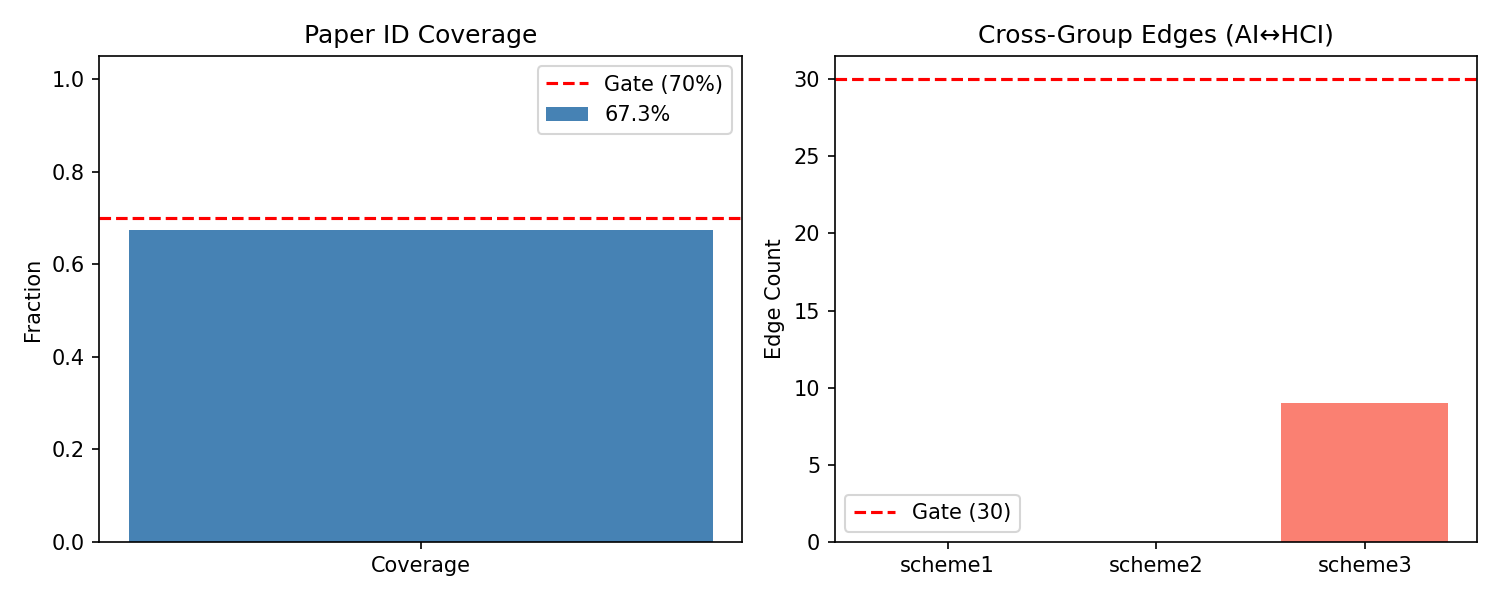
\includegraphics[width=\columnwidth]{figures/fig1_gate_metrics.png}
\caption{Gate evaluation results per classification scheme. Coverage rate (left panel) against the 70\% gate threshold; cross-group edge count (right panel) against the 30-edge threshold. Scheme 3 (FoS-primary) classifies all 33 resolved papers but yields only 9 cross-group edges at proxy corpus scale.}
\label{fig:gate}
\end{figure}

\begin{figure}[h]
\centering
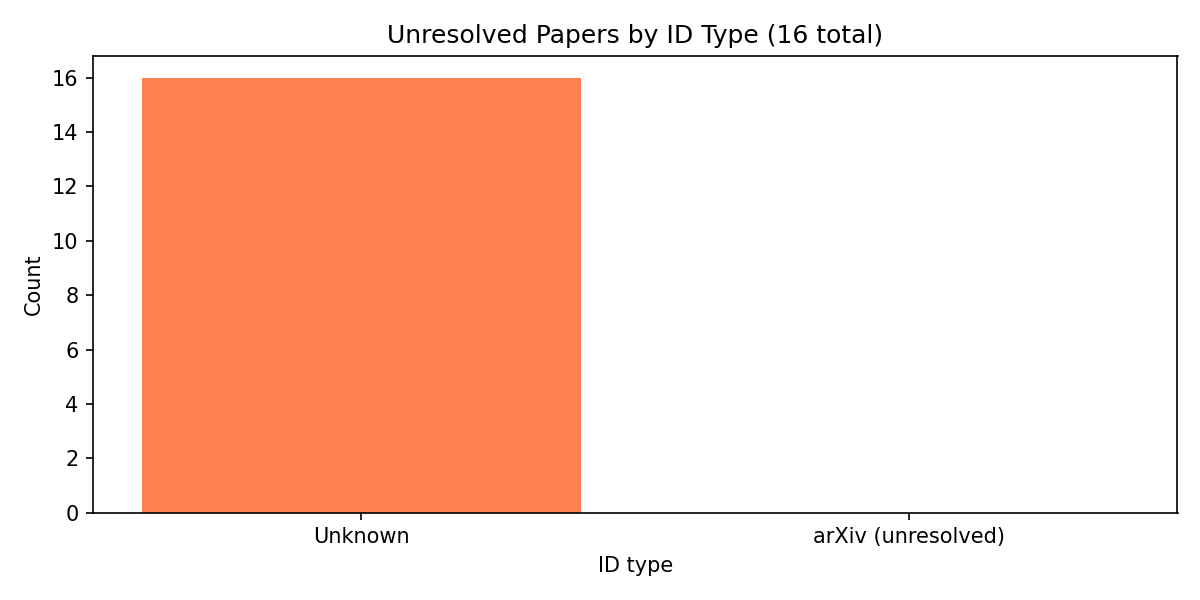
\includegraphics[width=\columnwidth]{figures/fig2_dropout_by_venue.png}
\caption{Unresolved papers by ID type and inferred source venue. 16 of 49 papers fail S2AG resolution because they are ACM DL publications without arXiv preprints. Dropout is non-systematic with respect to venue group, introducing no directional bias.}
\label{fig:dropout}
\end{figure}

\begin{figure}[h]
\centering
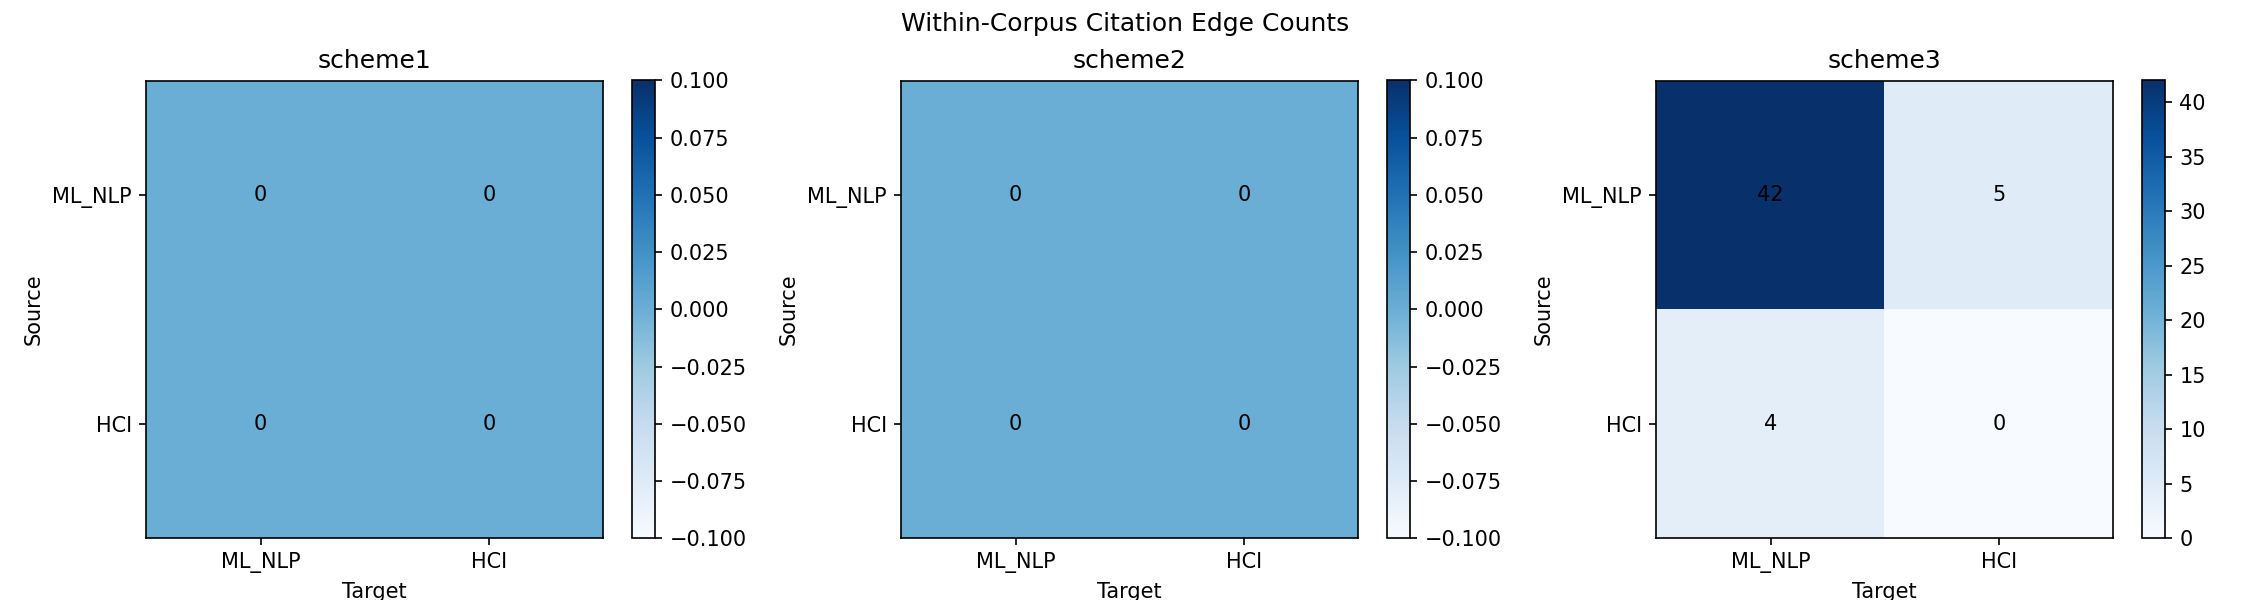
\includegraphics[width=\columnwidth]{figures/fig3_edge_heatmaps.png}
\caption{Directed citation edge count heatmaps for all three classification schemes. Scheme 3 (right panel): ML\_NLP$\to$ML\_NLP=42, ML\_NLP$\to$HCI=5, HCI$\to$ML\_NLP=4, HCI$\to$HCI=0. Asymmetry ratio = 0.107.}
\label{fig:heatmaps}
\end{figure}

\begin{figure}[h]
\centering
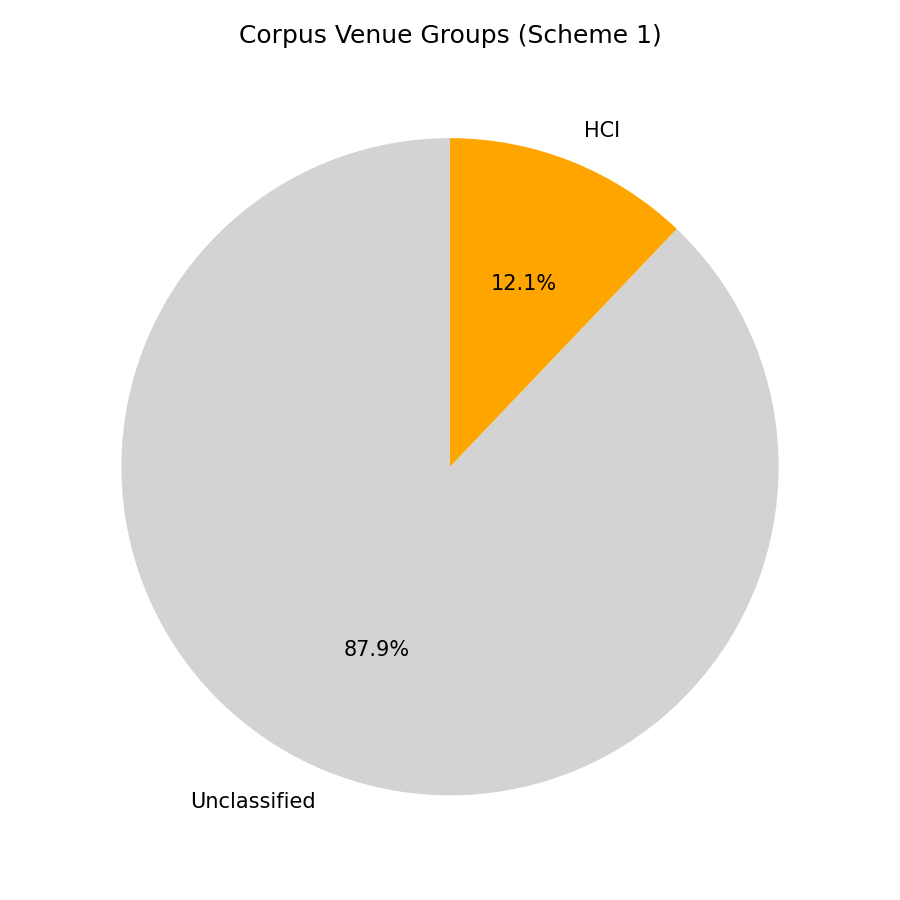
\includegraphics[width=\columnwidth]{figures/fig4_venue_pie.png}
\caption{Corpus composition by venue group under Scheme 1 (venue-string) classification. Only 4 of 33 resolved papers are classified, illustrating the 12\% coverage limitation.}
\label{fig:pie}
\end{figure}

\begin{figure}[h]
\centering
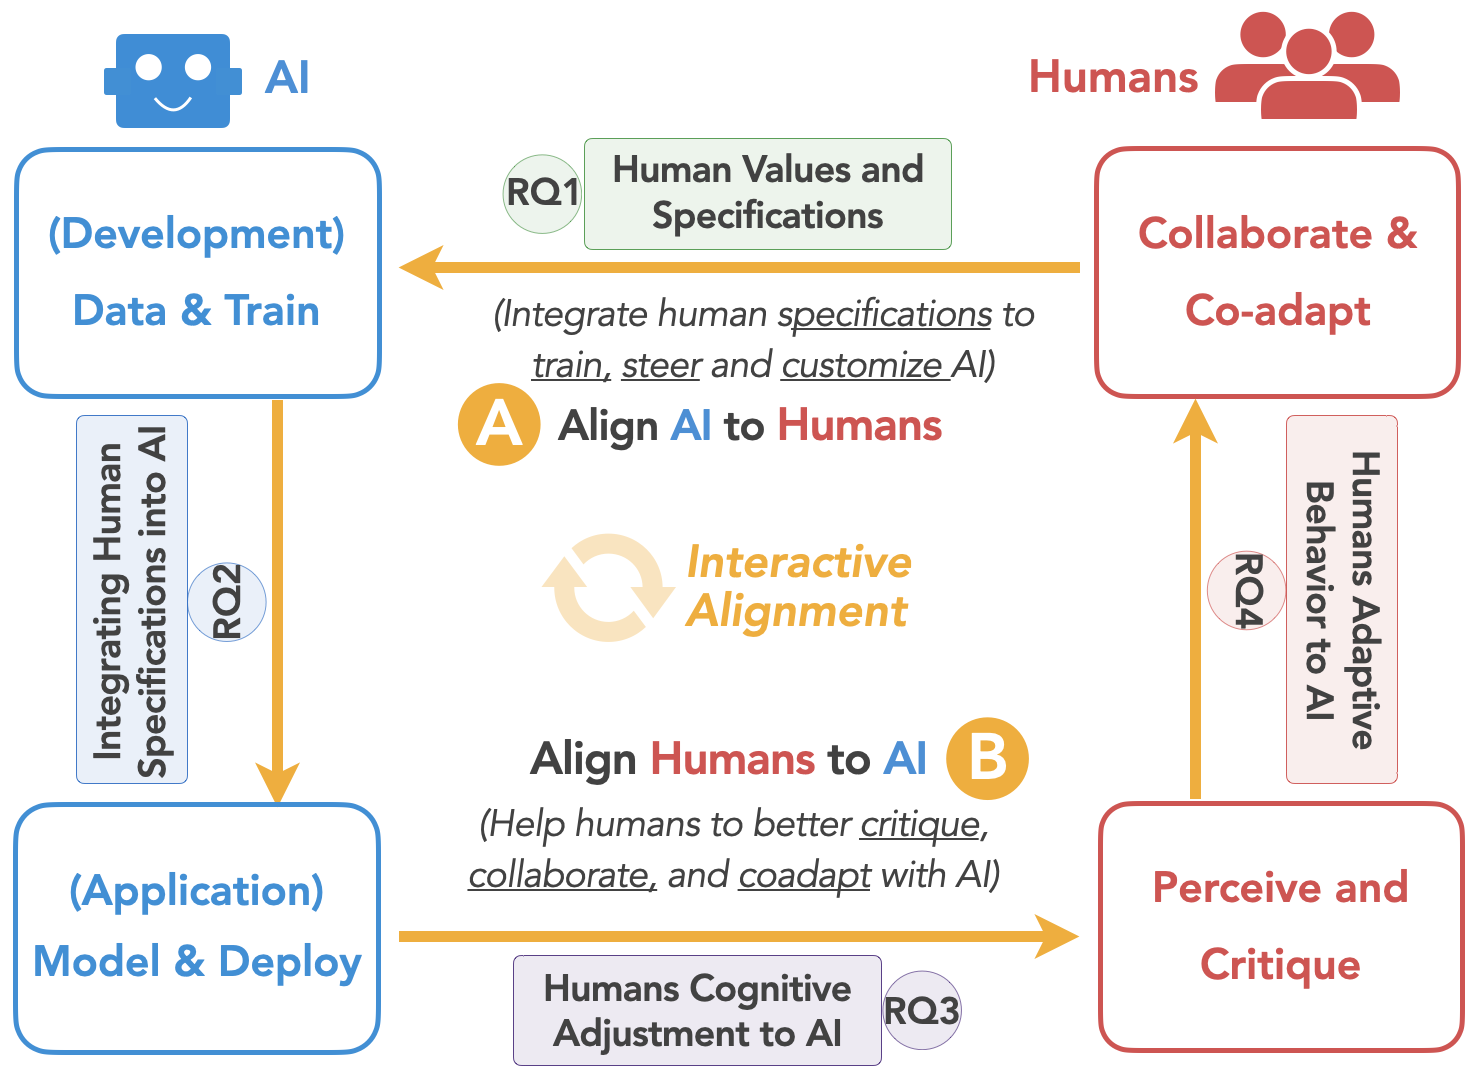
\includegraphics[width=\columnwidth]{figures/corpus_overview.png}
\caption{Overview of the huashen218 bidirectional alignment corpus structure as accessed via the public GitHub reading list. $\sim$130 linked papers yield 49 extractable identifiers and 33 S2AG-resolved papers.}
\label{fig:corpus}
\end{figure}
